%% ----------------------------------------------------------------
%% Article.tex
%% ---------------------------------------------------------------- 
\documentclass{ecsarticle}     % Use the Article Style
\graphicspath{{Figures/}}   % Location of your graphics files
\usepackage{natbib}            % Use Natbib style for the refs.
\hypersetup{colorlinks=false}   % Set to false for black/white printing
\input{Definitions}            % Include your abbreviations

\usepackage[nodayofweek]{datetime}
\usepackage{listings}
\usepackage{color}

\usepackage{graphicx}



%% ----------------------------------------------------------------
\begin{document}
\frontmatter
\title      {COMP6036: Advanced Machine Learning\\
            An investigation into DBSCAN}
      
\addresses  {\deptname\\\univname}
\authors                 {\href{mailto:ajr2g10@ecs.soton.ac.uk}{Ashley J. Robinson}\\\href{mailto:ajr2g10@ecs.soton.ac.uk}{ajr2g10@ecs.soton.ac.uk}}

\date       {\today}
\subject    {}
\keywords   {}
\maketitle
%% ----------------------------------------------------------------



\begin{abstract}
DBSCAN is used for clustering sparse spatial databases using data point density.
The algorithm performs well at this but has some shortcomings when applied to specific tasks.
Scalability is ones of its major advanatges.
\end{abstract}

\mainmatter


\section{Motivation for Algorithm}

DBSCAN (Density-Based Spatial Clustering of Applications with Noise) is an unsupervised application of machine learning introduced by~\cite{ester96dbscan}.
Intended to address Spatial Database Systems (SDBS) which can be produced from natural geometric and geographical datasets or applications such a layout for integrated circuit design~\citep{guting94sdbs}.
It has three main objectives.
To minimise the required domain knowledge needed to set input parameters, have the capability to discover clusters of arbitrary shapes and to perform well on large spatial databases.

At the time of creation the algorithms was compared to a recent development called CALARANS~\citep{ng94clarans} which is an extension of CLARA (Clustering LARge Applications)~\citep{kaufman90clara}.
Both algorithms are intended for use on large databases but CLARANS uses random noise to improve performance.
Apart from traditional clustering algorithms, such a K-means, DBSCAN was a breakthrough in terms of a density approach to datasets.

\section{Technical Explanation}

DBSCAN uses the notion of cluster density to classify data.
It is intuitive to build a community of data points by attempting to draw a path of connectivity.
This leads to the first input parameter to the algorithm, $\epsilon$, a distance threshold for which DBSCAN is permitted to move yet remain in the same cluster.
Equation~\eqref{eqn:dist}, adapted from~\cite{ester96dbscan}, is the basic function used to determine membership by thresholding; euclidean distance is used in this case but the measure of distance can be replaced with a Manhattan norm to scale down computational overheads~\citep{krause86taxicab}.

\newpage
\begin{equation}
	N(\textbf{p},\textbf{q},\epsilon) = \left\{
		\begin{array}{l}
    		1,\: ||\textbf{p} - \textbf{q}|| \leq \epsilon\\
    		0,\: ||\textbf{p} - \textbf{q}|| > \epsilon
  		\end{array} \right.
	\:\:where\:\: \textbf{q},\textbf{p} \in \textbf{D}
	\label{eqn:dist}
\end{equation}


This approach is simple for compact clusters but when noise is introduced the algorithm will identify a few points as a whole cluster.
A second threshold is introduced, however this is unnecessary to perform basic DBSCAN clustering, to set the minimum number of members a cluster can have.
This parameter, $\lambda$, if successfully applied to Equation~\eqref{eqn:inside} decides when to build a cluster around the point.
Equation~\eqref{eqn:member} takes the sum of connected datapoints attributed to single point used for comparison and outputs the number of all datapoints in the input space which are connected. 

\begin{equation}
	\lambda \leq C(\textbf{p},\epsilon) 
	\label{eqn:inside}
\end{equation}
\begin{equation}
	C(\textbf{p},\epsilon) = \sum\limits_{\textbf{q}\:\in\:\textbf{D}\atop\textbf{q}\:\neq\:\textbf{p}} N(\textbf{p},\textbf{q},\epsilon)
	\label{eqn:member}
\end{equation}

It is clear there is a lot of scope for optimisation in practice.
A list containing all datapoints at the start of the algorithm can be used to check off point which have been found to belong to a cluster.
This means for an input space containing $n$ clusters that can be perfectly segmented by DBSCAN requires only $n$ calls of Equation~\eqref{eqn:member}.

\begin{equation}
	C(\textbf{B},\textbf{p},\epsilon) = \sum\limits_{\textbf{q}\:\in\:\textbf{D}\atop\textbf{q}\:\neq\:\textbf{p}} N(\textbf{p},\textbf{q},\epsilon)
	\label{eqn:optimised}
\end{equation}

\section{Performance}

The graphs in Figure~\ref{fig:compare} are different clustering algorithms applied to a shape dataset taken from~\cite{gionis05cluster}. 
Algorithms were taken from a machine learning toolbox for Python~\citep{scikit13ml}.
The dataset contains seven clusters but in two cases there are \emph{bridges} between the clusters.
On the far right K-Means and WARD correctly divides the data where DBSCAN incorrectly groups both clusters together; shown in Figures~\ref{fig:kmeans},~\ref{fig:ward} and~\ref{fig:dbscan} respectively.
DBSCAN deals well with the remaining data where other two algorithms fail.
Centroid approaches leave large clusters divided due to nearby smaller clusters.


\begin{figure}[ht]
   \centering
   \subfigure[K-Means]{
      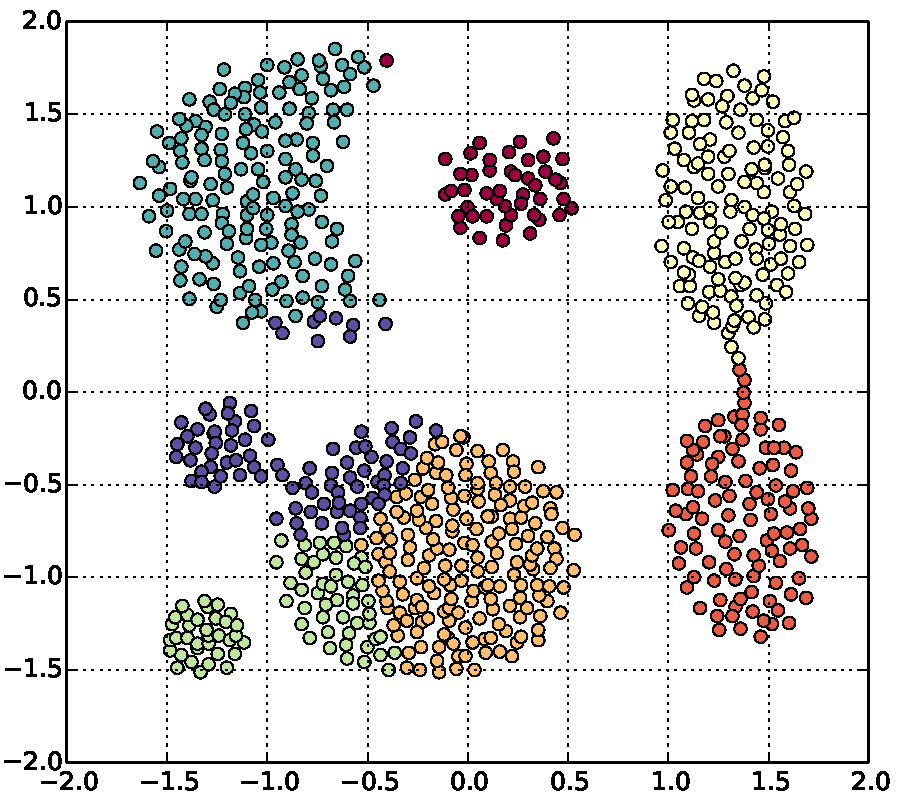
\includegraphics[height = 5cm,width = 5cm]{kmeans.pdf}
      \label{fig:kmeans}
   }
   \subfigure[WARD]{
      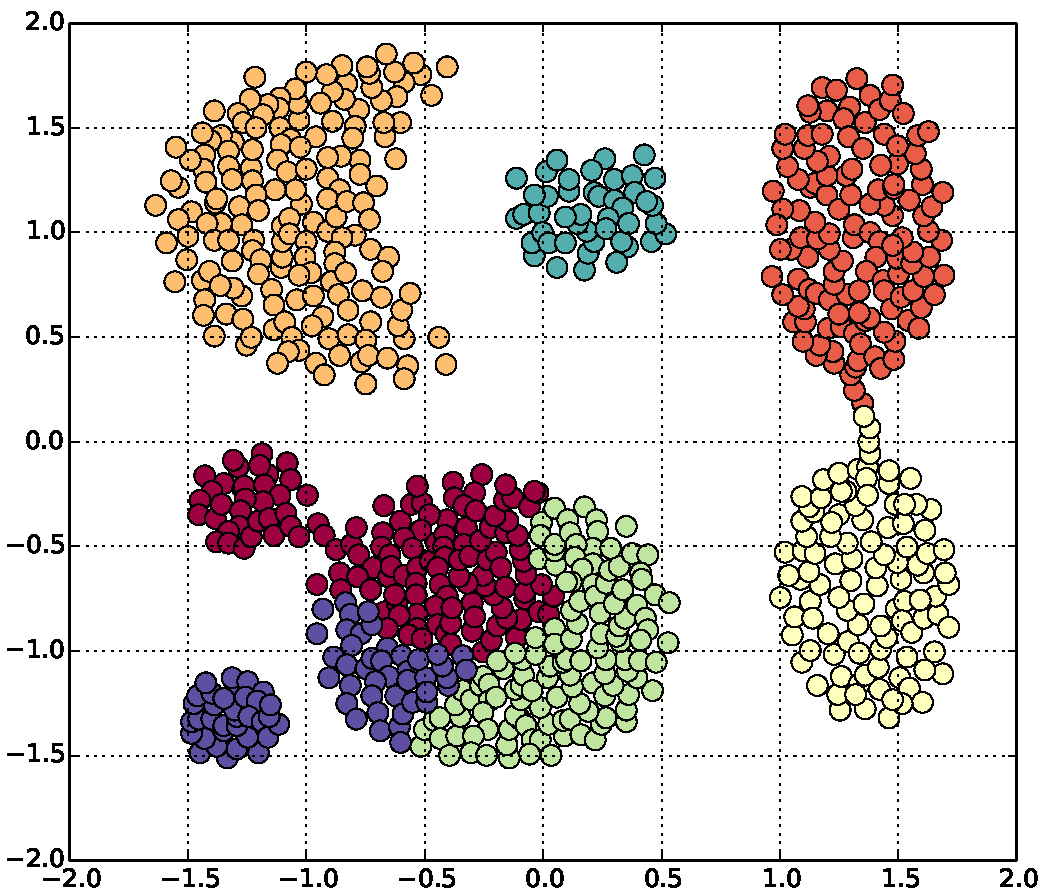
\includegraphics[height = 5cm, width = 5cm]{ward.pdf}
      \label{fig:ward}
   }
   \subfigure[DBSCAN]{
      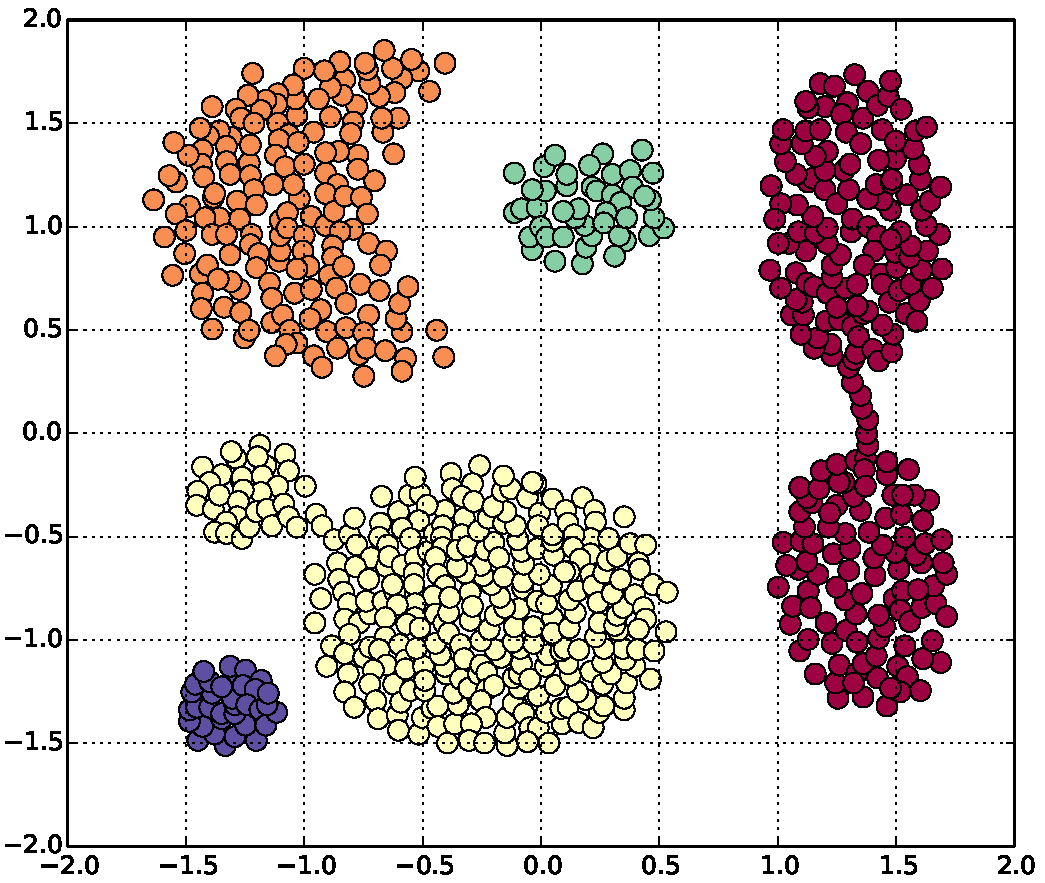
\includegraphics[height = 5cm,width = 5cm]{dbscan.pdf}
      \label{fig:dbscan}
   }
   \caption{A comparison against DBSCAN}
   \label{fig:compare}
\end{figure}

The algorithm exhibits variation in perforamce as per the standard bias-variance dilemma.
Figure~\ref{fig:error} shows how the error varies for DBSCAN when applied to data used in Figure~\ref{fig:compare}.
The EPS paramter sets the distance which the algorithm allow itself to jump and consider itself in the same cluster.

\begin{figure}[ht]
   \centering
    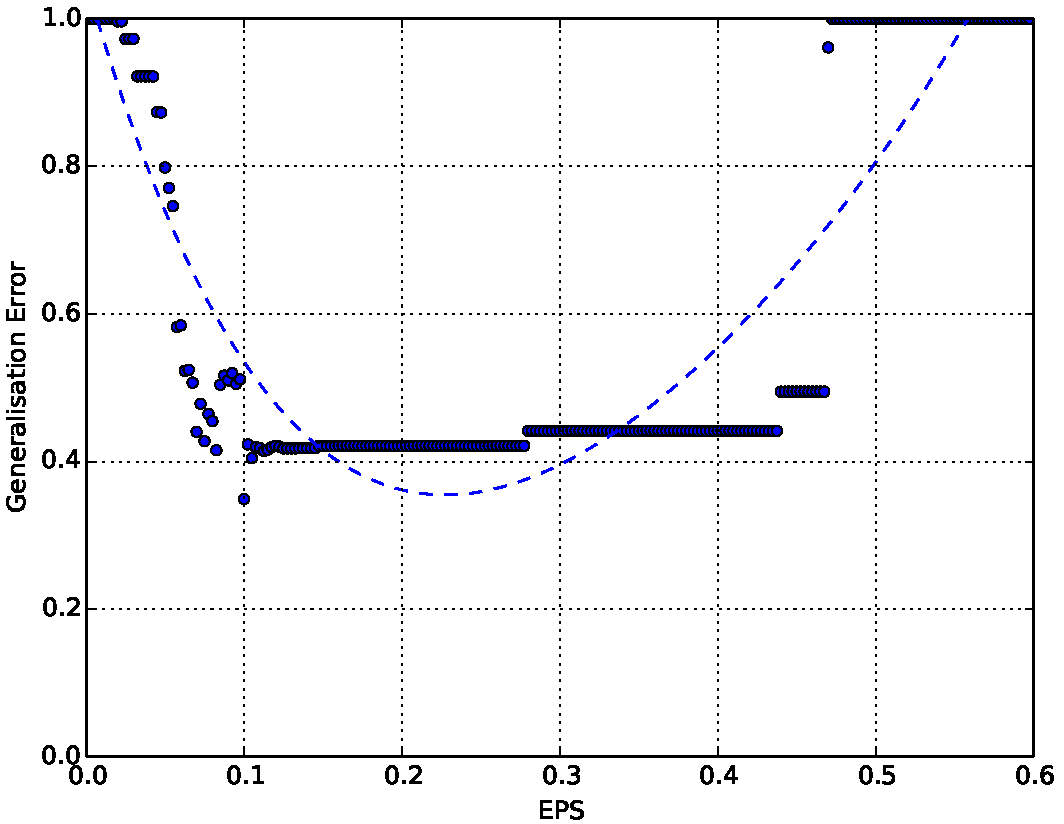
\includegraphics[height = 5cm,width = 8cm]{error.pdf}
   \caption{Generalisation error with varying input parameter}
   \label{fig:error}
\end{figure}




\section{Conclusion and Further Work}


\bibliographystyle{ecs}
\bibliography{references}



\end{document}
%% ----------------------------------------------------------------

